\section{Experimental Results and Evaluation}\label{sec:results}

This section evaluates the effectiveness and generalization of \scl{} against the host trackers
using identical detections and published tracker configurations. Section~\ref{sec:tracker}
examines tracking performance across different trackers on MOT17, while Sect.~\ref{sec:detector}
evaluates detector--tracker compatibility on KITTI. Section~\ref{sec:shift} investigates robustness
to detection confidence-score shifts, and Sect.~\ref{sec:baselines} compares \scl{} with adaptive
thresholding methods. Section~\ref{sec:ablation} presents component ablation and parameter
sensitivity analyses. Finally, Sects.~\ref{sec:external} and~\ref{sec:visdrone} assess
generalization to previously unseen trackers and the held-out UAVDT dataset, respectively. In all
comparisons, the baseline is the host tracker operating without \scl{}, and Fig.~\ref{fig:forest}
summarizes the HOTA differences across the evaluated configurations.

\emph{How to read the result tables.} Each result table compares two runs on the same detections:
A, the tracker alone (Host), and B, the same tracker with \scl{} (Host+\scl{}). HOTA, MOTA, and
IDF1 are percentages, and higher is better ($\uparrow$); IDS counts identity switches, and lower is
better ($\downarrow$). The column Change gives B minus A, so a positive change in HOTA, MOTA, or
IDF1 and a negative change in IDS mean that \scl{} helped. The brackets give the 95\% bootstrap
interval of the change: when the whole interval lies on one side of zero, the change is reliable
and printed in bold; when it includes zero, A and B are not reliably different. ``Identical'' means
that \scl{} did not change the tracker's output at all. For example, in Table~\ref{tab:kitti}
ByteTrack with RT-DETR-L has a MOTA of 47.27 alone and 53.24 with \scl{}; the change is $+5.98$
points, and its interval $[+1.16,+9.94]$ lies above zero, so the gain is reliable. Values are
rounded separately, so B minus A can differ from the change in the last digit.

\begin{figure}[!t]
\centering
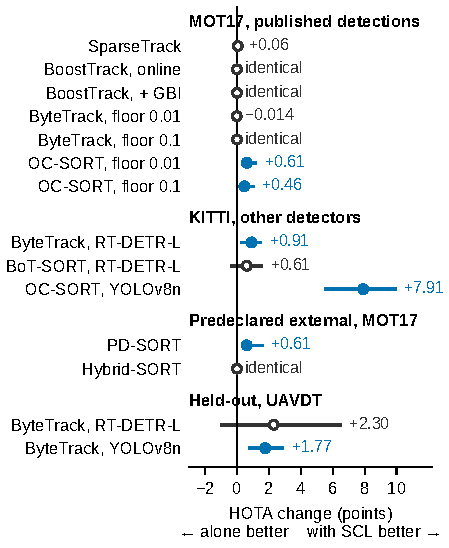
\includegraphics{Fig3.pdf}
\caption{Summary of all HOTA results: for every tested tracker and detector, how much \scl{}
changes HOTA (tracker with \scl{} minus tracker alone, in points). Dot and number: the change; line:
its 95\% bootstrap interval. Right of the vertical line at zero, \scl{} is better. Filled dot: a
reliable gain (the whole interval is above zero); open dot: no reliable change (the interval
includes zero) or identical output}
\label{fig:forest}
\end{figure}

\subsection{Performance Across Trackers on MOT17}\label{sec:tracker}
Table~\ref{tab:mot17} shows the development trackers on MOT17 val-half. The two-stage trackers with
well-matched detections stayed at the accuracy of their hosts: BoostTrack, online and with GBI, and
ByteTrack at floor 0.1 gave exactly the same output, and ByteTrack at floor 0.01 and SparseTrack
stayed within 0.06 HOTA points, the self-limiting clean mode. The single-stage OC-SORT improved at
both floors (HOTA from 66.43 to 67.04 and from 66.44 to 66.91, MOTA $+1.27$ and $+1.26$), with fewer identity switches and
higher HOTA on 7 of 7 sequences, through the continuation rescue.

\begin{table}[!tb]
\caption{MOT17 val-half with the published YOLOX-X detections: each development tracker alone and with \scl{}. Host: the tracker alone; Host+\scl{}: the same tracker with \scl{}, on the same detections. Change: Host+\scl{} minus Host, with its 95\% bootstrap interval in brackets; bold: the interval does not include zero, so the change is reliable. $\uparrow$: higher is better; $\downarrow$: lower is better (IDS: identity switches, a count). Paper: the number reported by the tracker's authors (--: not reported). Floor: the lowest detector score emitted.}
\label{tab:mot17}
\centering\footnotesize
\setlength{\tabcolsep}{2.5pt}
\begin{tabular}{@{}lrrrl@{}}
\toprule
Metric & Paper & Host & \begin{tabular}[b]{@{}r@{}}Host\\+\scl{}\end{tabular} & Change [95\% CI]\\
\midrule
\multicolumn{5}{@{}l}{\textit{SparseTrack} \cite{liu2025sparsetrack}}\\
\quad HOTA$\uparrow$ & 69.2 & 68.88 & 68.93 & $+0.06$ [$-0.01$, $+0.25$]\\
\quad MOTA$\uparrow$ & 76.8 & 77.85 & 77.93 & $+0.08$ [$-0.03$, $+0.30$]\\
\quad IDF1$\uparrow$ & 81.4 & 81.97 & 82.13 & $+0.16$ [$-0.02$, $+0.70$]\\
\quad IDS$\downarrow$ & -- & 124 & 131 & $+7$ [$0$, $+19$]\\
\multicolumn{5}{@{}l}{\textit{BoostTrack, online} \cite{stanojevic2024boosttrack}}\\
\quad HOTA$\uparrow$ & 68.37 & 68.49 & 68.49 & 0 (identical)\\
\quad MOTA$\uparrow$ & 75.56 & 75.50 & 75.50 & 0 (identical)\\
\quad IDF1$\uparrow$ & 81.35 & 81.41 & 81.41 & 0 (identical)\\
\quad IDS$\downarrow$ & 118 & 113 & 113 & 0 (identical)\\
\multicolumn{5}{@{}l}{\textit{BoostTrack, + GBI} \cite{stanojevic2024boosttrack}}\\
\quad HOTA$\uparrow$ & 71.33 & 71.73 & 71.73 & 0 (identical)\\
\quad MOTA$\uparrow$ & 80.55 & 81.03 & 81.03 & 0 (identical)\\
\quad IDF1$\uparrow$ & 83.84 & 84.16 & 84.16 & 0 (identical)\\
\quad IDS$\downarrow$ & 106 & 97 & 97 & 0 (identical)\\
\multicolumn{5}{@{}l}{\textit{ByteTrack, floor 0.01} \cite{zhang2022bytetrack}}\\
\quad HOTA$\uparrow$ & -- & 67.70 & 67.68 & $-0.014$ [$-0.058$, $+0.009$]\\
\quad MOTA$\uparrow$ & 76.6 & 77.60 & 77.66 & $+0.06$ [$-0.15$, $+0.34$]\\
\quad IDF1$\uparrow$ & 79.3 & 79.47 & 79.44 & $-0.031$ [$-0.135$, $+0.035$]\\
\quad IDS$\downarrow$ & -- & 214 & 218 & $+4$ [$-2$, $+13$]\\
\multicolumn{5}{@{}l}{\textit{ByteTrack, floor 0.1} \cite{zhang2022bytetrack}}\\
\quad HOTA$\uparrow$ & -- & 67.70 & 67.70 & 0 (identical)\\
\quad MOTA$\uparrow$ & 76.6 & 77.60 & 77.60 & 0 (identical)\\
\quad IDF1$\uparrow$ & 79.3 & 79.47 & 79.47 & 0 (identical)\\
\quad IDS$\downarrow$ & -- & 214 & 214 & 0 (identical)\\
\multicolumn{5}{@{}l}{\textit{OC-SORT, floor 0.01} \cite{cao2023ocsort}}\\
\quad HOTA$\uparrow$ & 66.5 & 66.43 & 67.04 & {\boldmath $+0.61$ [$+0.36$, $+1.24$]}\\
\quad MOTA$\uparrow$ & 74.9 & 74.67 & 75.94 & {\boldmath $+1.27$ [$+0.17$, $+3.01$]}\\
\quad IDF1$\uparrow$ & 77.7 & 78.05 & 78.71 & $+0.66$ [$-0.25$, $+1.60$]\\
\quad IDS$\downarrow$ & -- & 211 & 203 & {\boldmath $-8$ [$-15$, $-2$]}\\
\multicolumn{5}{@{}l}{\textit{OC-SORT, floor 0.1} \cite{cao2023ocsort}}\\
\quad HOTA$\uparrow$ & 66.5 & 66.44 & 66.91 & {\boldmath $+0.46$ [$+0.27$, $+1.09$]}\\
\quad MOTA$\uparrow$ & 74.9 & 74.67 & 75.93 & {\boldmath $+1.26$ [$+0.37$, $+3.34$]}\\
\quad IDF1$\uparrow$ & 77.7 & 78.05 & 78.33 & {\boldmath $+0.287$ [$+0.003$, $+0.838$]}\\
\quad IDS$\downarrow$ & -- & 213 & 199 & $-14$ [$-38$, $+6$]\\
\bottomrule
\end{tabular}
\end{table}


\subsection{Cross-Detector Evaluation on KITTI}\label{sec:detector}
\begin{figure*}[t]
\centering
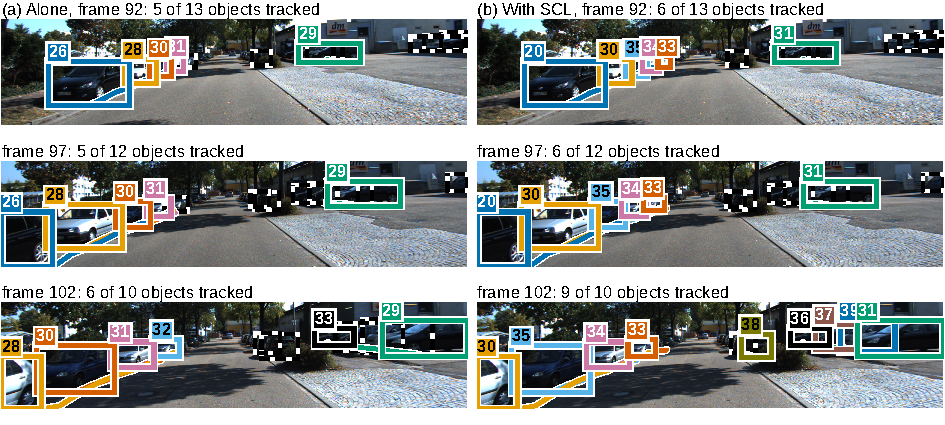
\includegraphics{Fig4.pdf}
\caption{The same video tracked twice: KITTI sequence 0001 \cite{geiger2012kitti} with OC-SORT
and YOLOv8n, at frames 92, 97, and 102 (rows). (a) The tracker alone; (b) the same tracker with
\scl{}. Each colour and number is one track (one object identity); its line shows where the object
was in the previous 20 frames. Dashed boxes: labelled objects that no track follows (missed). At
frame 102, the tracker alone follows 6 of the 10 labelled objects and with \scl{} 9. IDs are
numbered separately in each run. This sequence has the median HOTA gain of the 21 sequences, and frame 102 is its first frame with
the largest gain in tracked objects}
\label{fig:example}
\end{figure*}
Table~\ref{tab:kitti} shows what happens when the detector is replaced. With the noisy RT-DETR-L,
ByteTrack gained 5.98 MOTA, 3.87 IDF1, and 0.91 HOTA points, and BoT-SORT 7.86 MOTA, 3.10 IDF1,
and 0.61 HOTA points, with 297 and 226 fewer identity switches. With YOLOv8n, OC-SORT rose from 36.27 to 44.18
HOTA ($+7.91$ points, $[+5.47,+9.98]$), 9.40 MOTA points, and 9.60 IDF1 points; it followed many more objects, as
its missed objects (FN) fell by 5,310, and its identity switches rose with them by 79.
Fig.~\ref{fig:example} follows this cell over three frames: each object keeps its ID,
and at frame 102 OC-SORT alone tracked 6 of the 10 labelled objects and with \scl{} 9.

\begin{table}[!tb]
\caption{KITTI tracking training with detectors that the trackers were not tuned for (HOTA averaged over cars and pedestrians). Host: the tracker alone; Host+\scl{}: the same tracker with \scl{}, on the same detections. Change: Host+\scl{} minus Host, with its 95\% bootstrap interval in brackets; bold: the interval does not include zero, so the change is reliable. $\uparrow$: higher is better; $\downarrow$: lower is better (IDS: identity switches, a count). BoT-SORT: sequence 0020 is left out of both runs, because the BoT-SORT code stops with a numerical error on it.}
\label{tab:kitti}
\centering\footnotesize
\setlength{\tabcolsep}{2.5pt}
\begin{tabular}{@{}lrrl@{}}
\toprule
Metric & Host & \begin{tabular}[b]{@{}r@{}}Host\\+\scl{}\end{tabular} & Change [95\% CI]\\
\midrule
\multicolumn{4}{@{}l}{\textit{ByteTrack} \cite{zhang2022bytetrack}\textit{, RT-DETR-L}}\\
\quad HOTA$\uparrow$ & 50.73 & 51.64 & {\boldmath $+0.91$ [$+0.22$, $+1.55$]}\\
\quad MOTA$\uparrow$ & 47.27 & 53.24 & {\boldmath $+5.98$ [$+1.16$, $+9.94$]}\\
\quad IDF1$\uparrow$ & 64.98 & 68.86 & {\boldmath $+3.87$ [$+1.67$, $+5.06$]}\\
\quad IDS$\downarrow$ & 686 & 389 & {\boldmath $-297$ [$-530$, $-122$]}\\
\multicolumn{4}{@{}l}{\textit{BoT-SORT} \cite{aharon2022botsort}\textit{, RT-DETR-L} (20 sequences)}\\
\quad HOTA$\uparrow$ & 53.91 & 54.52 & $+0.61$ [$-0.39$, $+1.61$]\\
\quad MOTA$\uparrow$ & 48.25 & 56.11 & {\boldmath $+7.86$ [$+2.21$, $+13.44$]}\\
\quad IDF1$\uparrow$ & 67.74 & 70.85 & {\boldmath $+3.10$ [$+1.00$, $+4.57$]}\\
\quad IDS$\downarrow$ & 476 & 250 & {\boldmath $-226$ [$-369$, $-120$]}\\
\multicolumn{4}{@{}l}{\textit{OC-SORT} \cite{cao2023ocsort}\textit{, YOLOv8n}}\\
\quad HOTA$\uparrow$ & 36.27 & 44.18 & {\boldmath $+7.91$ [$+5.47$, $+9.98$]}\\
\quad MOTA$\uparrow$ & 33.99 & 43.39 & {\boldmath $+9.40$ [$+1.10$, $+12.30$]}\\
\quad IDF1$\uparrow$ & 50.46 & 60.05 & {\boldmath $+9.60$ [$+5.61$, $+12.16$]}\\
\quad IDS$\downarrow$ & 91 & 170 & {\boldmath $+79$ [$+43$, $+125$]}\\
\bottomrule
\end{tabular}
\end{table}

\begin{table}[!tb]
\caption{MOT17 val-half with the detector scores changed before the tracker, while the tracker keeps its published thresholds: $s^3$ cubes every score, $0.5\,s$ halves it, and $T=2$ and $T=0.5$ divide its logit by 2 or by 0.5. HOTA (\%, higher is better) of the tracker alone (Host) and with \scl{} (Host+\scl{}); 0.00 means that no object was tracked. Change: Host+\scl{} minus Host, with its 95\% bootstrap interval; bold: the interval does not include zero (a reliable change). Lowest emitted score 0.01 (BoostTrack 0.1).}
\label{tab:shift}
\centering\footnotesize
\setlength{\tabcolsep}{3pt}
\begin{tabular}{@{}lrrl@{}}
\toprule
 & \multicolumn{3}{c}{HOTA (\%)}\\
\cmidrule(l){2-4}
Score change & Host & \begin{tabular}[b]{@{}r@{}}Host\\+\scl{}\end{tabular} & Change [95\% CI]\\
\midrule
\multicolumn{4}{@{}l}{\textit{ByteTrack, official setting} \cite{zhang2022bytetrack}}\\
\quad $s^3$ & 60.92 & 65.81 & {\boldmath $+4.89$ [$+2.60$, $+13.69$]}\\
\quad $0.5\,s$ & 0.00 & 66.17 & {\boldmath $+66.17$ [$+49.32$, $+75.40$]}\\
\quad $T=2$ & 65.84 & 66.95 & {\boldmath $+1.11$ [$+0.35$, $+3.87$]}\\
\quad $T=0.5$ & 67.30 & 67.29 & $-0.009$ [$-0.051$, $+0.005$]\\
\multicolumn{4}{@{}l}{\textit{ByteTrack, library setting} \cite{zhang2022bytetrack}}\\
\quad $s^3$ & 66.31 & 66.31 & $-0.006$ [$-0.384$, $+0.383$]\\
\quad $0.5\,s$ & 66.61 & 66.48 & $-0.14$ [$-0.66$, $+0.14$]\\
\quad $T=2$ & 63.97 & 63.97 & 0 (identical)\\
\quad $T=0.5$ & 66.53 & 66.53 & $-0.006$ [$-0.029$, $+0.001$]\\
\multicolumn{4}{@{}l}{\textit{OC-SORT} \cite{cao2023ocsort}}\\
\quad $s^3$ & 58.34 & 66.60 & {\boldmath $+8.26$ [$+5.86$, $+16.81$]}\\
\quad $0.5\,s$ & 0.00 & 66.72 & {\boldmath $+66.72$ [$+50.32$, $+75.56$]}\\
\quad $T=2$ & 65.99 & 67.22 & {\boldmath $+1.24$ [$+0.52$, $+3.42$]}\\
\quad $T=0.5$ & 66.61 & 67.06 & $+0.45$ [$-0.01$, $+0.97$]\\
\multicolumn{4}{@{}l}{\textit{BoostTrack, online} \cite{stanojevic2024boosttrack}}\\
\quad $s^3$ & 61.33 & 64.84 & {\boldmath $+3.51$ [$+0.85$, $+13.28$]}\\
\quad $T=2$ & 67.59 & 67.59 & 0 (identical)\\
\bottomrule
\end{tabular}
\end{table}

\begin{table}[!tb]
\caption{KITTI tracking training: HOTA (\%, higher is better) of the tracker alone (Host), of two simple adaptive baselines ($t_1$, $t_2$), and of \scl{}, on the same detections. In the baselines, the tracker's thresholds are set in every frame to the first ($t_1$) or second ($t_2$) Otsu split of the logits of the last 10 frames, and the scores are not changed. Halved: halved detector scores. \scl{} $-$ $t_2$: the gain of \scl{} over the stronger baseline, with its 95\% bootstrap interval below; bold: the interval does not include zero (a reliable gain).}
\label{tab:baselines}
\centering\footnotesize
\setlength{\tabcolsep}{3pt}
\begin{tabular}{@{}lrrrrc@{}}
\toprule
Cell & Host & $t_1$ & $t_2$ & \scl{} & \scl{} $-$ $t_2$\\
\midrule
\twol{OC-SORT,}{YOLOv8n} & 36.27 & 39.97 & 41.09 & 44.18 & \cib{+3.09}{+2.00}{+4.03}\\
\addlinespace[3pt]
\begin{tabular}[c]{@{}l@{}}ByteTrack,\\RT-DETR-L,\\halved\end{tabular} & 49.50 & 49.58 & 49.50 & 51.79 & \cib{+2.29}{+0.28}{+4.96}\\
\addlinespace[3pt]
\begin{tabular}[c]{@{}l@{}}OC-SORT,\\YOLOv8n,\\halved\end{tabular} & 0.00 & 37.68 & 43.56 & 46.30 & \cib{+2.74}{+1.32}{+3.34}\\
\bottomrule
\end{tabular}
\end{table}

\begin{table*}[!tp]
\caption{ACT \cite{act2026adaptive} and \scl{} on the same detections and tracker. (a) HOTA in every tested setting. ACT, \scl{}: HOTA (\%, higher is better) of the tracker with each method. \scl{} $-$ ACT: how much higher \scl{} is than ACT in HOTA and in IDF1, with its 95\% bootstrap interval below. (b) MOTA and identity switches on UAVDT: the value with each method and \scl{} $-$ ACT with its 95\% bootstrap interval in brackets. A positive HOTA, IDF1, or MOTA difference and a negative IDS difference mean that \scl{} is better; bold: the interval does not include zero (a reliable difference). $\uparrow$: higher is better; $\downarrow$: lower is better (IDS: identity switches, a count). ACT uses its published parameters, without tuning. KITTI: HOTA averaged over cars and pedestrians; MOT17: val-half, the setting ACT was designed for; UAVDT: test split, one vehicle class, ignored regions removed (Sect.~\ref{sec:metrics}).}
\label{tab:act}
\centering\footnotesize
\setlength{\tabcolsep}{5pt}
{\textit{(a) HOTA and IDF1}}\par\smallskip
\begin{tabular}{@{}lllrrcc@{}}
\toprule
Data & Detector & Tracker & ACT & \scl{} & \scl{} $-$ ACT, HOTA & \scl{} $-$ ACT, IDF1\\
\midrule
KITTI, halved scores & RT-DETR-L & ByteTrack & 49.77 & 51.79 & \cib{+2.01}{+0.01}{+4.76} & \ci{+1.70}{-1.13}{+6.80}\\
KITTI, halved scores & YOLOv8n & OC-SORT & 36.24 & 46.30 & \cib{+10.06}{+6.88}{+12.01} & \cib{+12.03}{+6.85}{+14.69}\\
\addlinespace[4pt]
MOT17, floor 0.01 & YOLOX-X & ByteTrack (official) & 67.46 & 67.68 & \ci{+0.22}{-0.43}{+0.88} & \ci{+0.57}{-0.68}{+2.12}\\
MOT17, floor 0.1 & YOLOX-X & ByteTrack (official) & 67.46 & 67.70 & \ci{+0.23}{-0.40}{+0.90} & \ci{+0.60}{-0.55}{+2.10}\\
\addlinespace[4pt]
UAVDT test & YOLOv8n & ByteTrack & 29.01 & 30.83 & \cib{+1.82}{+0.65}{+3.00} & \cib{+4.00}{+1.85}{+6.22}\\
UAVDT test & RT-DETR-L & ByteTrack & 40.14 & 42.37 & \ci{+2.23}{-0.97}{+6.32} & \ci{+5.35}{-0.03}{+12.47}\\
\bottomrule
\end{tabular}

\medskip
{\textit{(b) MOTA and identity switches on UAVDT (test split, ByteTrack)}}\par\smallskip
\begin{tabular}{@{}lrrlrrl@{}}
\toprule
 & \multicolumn{3}{c}{MOTA$\uparrow$} & \multicolumn{3}{c}{IDS$\downarrow$}\\
\cmidrule(lr){2-4}\cmidrule(l){5-7}
Detector & ACT & \scl{} & \scl{} $-$ ACT [95\% CI] & ACT & \scl{} & \scl{} $-$ ACT [95\% CI]\\
\midrule
YOLOv8n & 16.59 & 17.29 & $+0.71$ [$-1.42$, $+2.52$] & 578 & 393 & $-185$ [$-480$, $+13$]\\
RT-DETR-L & 5.34 & 27.99 & {\boldmath $+22.65$ [$+9.03$, $+47.21$]} & 873 & 455 & {\boldmath $-418$ [$-718$, $-123$]}\\
\bottomrule
\end{tabular}
\end{table*}

\begin{table}[!tb]
\caption{What each part and each fixed value of \scl{} contributes, on KITTI (HOTA, \%, higher is better). First row: the HOTA of the frozen \scl{}. Every other row changes one thing only and gives the change in HOTA from the first row, in points: a negative value means that the version without that part, or with that value, is worse than the frozen \scl{}. In brackets: the frozen value. (a) OC-SORT, YOLOv8n; (b) ByteTrack, RT-DETR-L, halved scores; (c) OC-SORT, YOLOv8n, halved scores.}
\label{tab:compabl}
\centering\footnotesize
\setlength{\tabcolsep}{4pt}
\begin{tabular}{@{}lrrr@{}}
\toprule
Variant & (a) & (b) & (c)\\
\midrule
\scl{} (frozen) & 44.18 & 51.79 & 46.30\\
\addlinespace[2pt]
\multicolumn{4}{@{}l}{\textit{Ablation: one part removed}}\\
No weak detection recovery & $-3.35$ & $+0.06$ & $-1.16$\\
No remap (raw scores) & $0.00$ & $-1.67$ & $-0.61$\\
Always clean (no noisy mode) & $+0.15$ & $-2.40$ & $-2.44$\\
Always noisy (no clean mode) & $+0.08$ & $+0.24$ & $+0.85$\\
No background check & $-0.02$ & $+0.08$ & $+0.15$\\
Overlap-only duplicate rule & $+0.06$ & $+0.13$ & $-0.03$\\
No motion tolerance & $-0.10$ & $-0.04$ & $-0.14$\\
\addlinespace[2pt]
\multicolumn{4}{@{}l}{\textit{Sensitivity: one value changed (frozen value)}}\\
Window $W=5$ (10) & $+0.22$ & $-0.47$ & $-0.48$\\
Window $W=20$ (10) & $+0.56$ & $-0.04$ & $+0.26$\\
Mode median, last 100 frames (all) & $+0.18$ & $-0.19$ & $0.00$\\
Mode median, last 300 frames (all) & $+0.07$ & $+0.12$ & $+0.36$\\
Duplicate and recovery IoU 0.4 (0.5) & $+0.19$ & $+0.16$ & $-0.35$\\
Duplicate and recovery IoU 0.6 (0.5) & $-0.62$ & $-0.34$ & $-0.46$\\
Motion history 50 (100 frames) & $-0.05$ & $+0.06$ & $-0.09$\\
Motion history 200 (100 frames) & $+0.02$ & $+0.08$ & $+0.04$\\
\bottomrule
\end{tabular}
\end{table}

\begin{table}[!tb]
\caption{The two external trackers, chosen before the run and not used during design (MOT17 val-half, the authors' detections), each run once with the frozen \scl{}. Host: the tracker alone; Host+\scl{}: the same tracker with \scl{}, on the same detections. Change: Host+\scl{} minus Host, with its 95\% bootstrap interval in brackets; bold: the interval does not include zero, so the change is reliable. $\uparrow$: higher is better; $\downarrow$: lower is better (IDS: identity switches, a count). Paper: the number reported by the authors (for PD-SORT, their released output; --: not reported). EXACT: our Host within 0.2 HOTA of the authors' number; CLOSE: within 1.0.}
\label{tab:external}
\centering\footnotesize
\setlength{\tabcolsep}{2.5pt}
\begin{tabular}{@{}lrrrl@{}}
\toprule
Metric & Paper & Host & \begin{tabular}[b]{@{}r@{}}Host\\+\scl{}\end{tabular} & Change [95\% CI]\\
\midrule
\multicolumn{5}{@{}l}{\textit{PD-SORT} \cite{wang2025pdsort}\textit{, EXACT}}\\
\quad HOTA$\uparrow$ & 68.01 & 68.01 & 68.62 & {\boldmath $+0.61$ [$+0.27$, $+1.65$]}\\
\quad MOTA$\uparrow$ & 75.19 & 75.19 & 76.31 & {\boldmath $+1.13$ [$+0.27$, $+3.03$]}\\
\quad IDF1$\uparrow$ & 81.03 & 81.03 & 81.85 & {\boldmath $+0.82$ [$+0.43$, $+1.94$]}\\
\quad IDS$\downarrow$ & -- & 129 & 131 & $+2$ [$-9$, $+13$]\\
\multicolumn{5}{@{}l}{\textit{Hybrid-SORT} \cite{yang2024hybridsort}\textit{, CLOSE}}\\
\quad HOTA$\uparrow$ & 67.1 & 66.70 & 66.70 & 0 (identical)\\
\quad MOTA$\uparrow$ & 75.8 & 75.52 & 75.52 & 0 (identical)\\
\quad IDF1$\uparrow$ & 78.0 & 77.56 & 77.56 & 0 (identical)\\
\quad IDS$\downarrow$ & -- & 259 & 259 & 0 (identical)\\
\bottomrule
\end{tabular}
\end{table}

\begin{table}[!tb]
\caption{The held-out UAVDT test split (20 drone videos, not used during design), run once with the frozen \scl{}; ByteTrack with its published setting. Host: the tracker alone; Host+\scl{}: the same tracker with \scl{}, on the same detections. Change: Host+\scl{} minus Host, with its 95\% bootstrap interval in brackets; bold: the interval does not include zero, so the change is reliable. $\uparrow$: higher is better; $\downarrow$: lower is better (IDS: identity switches, a count).}
\label{tab:visdrone}
\centering\footnotesize
\setlength{\tabcolsep}{2.5pt}
\begin{tabular}{@{}lrrl@{}}
\toprule
Metric & Host & \begin{tabular}[b]{@{}r@{}}Host\\+\scl{}\end{tabular} & Change [95\% CI]\\
\midrule
\multicolumn{4}{@{}l}{\textit{ByteTrack, RT-DETR-L} \cite{zhang2022bytetrack,zhao2024rtdetr}}\\
\quad HOTA$\uparrow$ & 40.07 & 42.37 & $+2.30$ [$-1.05$, $+6.55$]\\
\quad MOTA$\uparrow$ & 3.29 & 27.99 & {\boldmath $+24.70$ [$+10.06$, $+51.08$]}\\
\quad IDF1$\uparrow$ & 48.59 & 54.33 & {\boldmath $+5.74$ [$+0.13$, $+13.11$]}\\
\quad IDS$\downarrow$ & 1041 & 455 & {\boldmath $-586$ [$-951$, $-248$]}\\
\multicolumn{4}{@{}l}{\textit{ByteTrack, YOLOv8n} \cite{zhang2022bytetrack,jocher2023yolov8}}\\
\quad HOTA$\uparrow$ & 29.05 & 30.83 & {\boldmath $+1.77$ [$+0.70$, $+2.94$]}\\
\quad MOTA$\uparrow$ & 16.27 & 17.29 & $+1.02$ [$-1.06$, $+2.86$]\\
\quad IDF1$\uparrow$ & 34.52 & 38.49 & {\boldmath $+3.97$ [$+1.88$, $+6.17$]}\\
\quad IDS$\downarrow$ & 719 & 393 & {\boldmath $-326$ [$-691$, $-73$]}\\
\bottomrule
\end{tabular}
\end{table}


\subsection{Robustness to Detection Score Shifts}\label{sec:shift}
Table~\ref{tab:shift} shows the trackers under the four score transforms. Halving the scores
reduced ByteTrack (official setting) and OC-SORT to 0 HOTA; with the layer they reached 66.17 and
66.72. Cubing reduced them to 60.92 and 58.34, and the layer restored them to 65.81 and 66.60;
BoostTrack rose from 61.33 to 64.84. With $T=2$, the layer raised ByteTrack and OC-SORT by 1.11 and
1.24 points. The library setting of ByteTrack, whose low thresholds already accept the changed
scores, stayed within 0.14 points. Over the 14 conditions, the layer raised HOTA significantly in 7
and lowered it significantly in none.


\subsection{Comparison with Adaptive Thresholding Methods}\label{sec:baselines}
Two simple baselines set the tracker's matching and birth thresholds in every frame to the first or
second Otsu split of the logits of the last 10 frames, $t_1$ or $t_2$, and pass the scores
unchanged. On KITTI (Table~\ref{tab:baselines}), \scl{} reached the highest HOTA in all three
cells, 2.2 to 8.6 points above the baselines, with intervals against the $t_2$ baseline above zero
in every cell, so adaptive thresholds alone do not explain the gains.

\emph{Logit-to-score conversion.} The baselines and \scl{} find their splits on logits, while a
tracker compares its thresholds with scores, so a split must be converted back with the logistic
function: the baselines pass $\sigma(t_1)$ or $\sigma(t_2)$ to the tracker, and \scl{} passes
$\min(a,\sigma(t_2))$ in clean frames (Eq.~\eqref{eq:clean}) and 0.5 with remapped scores in noisy
frames. The thresholds recorded in every frame matched these values exactly, with zero difference,
in every frame with a split of all eight baseline runs (7,987 frames with RT-DETR-L and 7,940
with YOLOv8n per run) and in all clean and noisy frames of \scl{} in the four KITTI cells. The baselines therefore received the thresholds they were meant to have.

\emph{ACT.} ACT \cite{act2026adaptive} is the closest published method: in every frame it sets
ByteTrack's high and low thresholds from the first quartile and the number of the current scores,
choosing between preset levels. It works on the scores directly, so it needs no conversion, and
under halved scores it receives the halved scores, as \scl{} does. It was run with its published
parameters, without retuning, on the same detections and hosts as \scl{} (Table~\ref{tab:act}):
its high threshold became the host's matching threshold and its low threshold the lower bound of
the second step, while the host's birth threshold and matching tolerance stayed unchanged; with
OC-SORT, which has one threshold, the high threshold served as that threshold. Before the
comparison, the ACT runner was run with the host's own thresholds and reproduced the output of the
host alone exactly in all 84 KITTI, 14 MOT17, and 40 UAVDT sequence runs. \scl{} reached higher HOTA
than ACT in every row of Table~\ref{tab:act}a, significantly under halved
scores ($+2.01$ and $+10.06$ points) and with YOLOv8n on UAVDT ($+1.82$), and also in the MOT17
setting for which ACT was designed. On UAVDT (Table~\ref{tab:act}b), \scl{} also reached a higher
MOTA and had fewer identity switches than ACT with both detectors. With RT-DETR-L its MOTA was 27.99
against 5.34 ($+22.65$, $[+9.03,+47.21]$), with 418 fewer identity switches, because the fixed score
levels of ACT removed few of the host's false positives. In no tested cell, including the two KITTI cells with the
original scores, was the HOTA of \scl{} significantly below that of ACT.

\subsection{Component Ablation and Parameter Sensitivity}\label{sec:ablation}
Table~\ref{tab:compabl} removes one part of the frozen \scl{}, or changes one of its values, at a
time on the three KITTI cells of Table~\ref{tab:baselines}, with the same detections and trackers.
Each part matters where its step acts. Without the weak detection recovery, the single-stage
OC-SORT lost 3.35 and 1.16 HOTA points, as it has no low-score step of its own. Without the noisy
mode (always clean), the halved-score cells lost 2.40 and 2.44 points, and without the remap up to
1.67 points. Always acting in the noisy mode stayed within 0.85 points of \scl{} on these KITTI
streams, which are noisy in most of their frames; on well-matched MOT17 trackers, however, always
acting is the earlier design \aob{}, which lowered HOTA by 4.15 to 5.89 points
(Table~\ref{tab:prior}). The mode decision is thus what lets one configuration serve both kinds of
stream. The background check, the duplicate rule, and the motion tolerance changed HOTA by at most
0.15 points on KITTI.

The sensitivity analysis, planned before the runs, changed the window $W$, the frames whose median
decides the mode, the IoU of the duplicate and recovery rules, and the motion history. For every
value and cell, HOTA stayed within 0.62 points of the frozen \scl{}, and within 0.24 points on the
fourth KITTI cell, ByteTrack with the original RT-DETR-L scores. The frozen values lie on a flat
part of the response, so none of them needs tuning for these detectors and trackers. The shorter
median windows, which bound the delay of the mode (Sect.~\ref{sec:regimes}), changed HOTA by at most
0.36 points on these streams.


\subsection{Generalization to Unseen Trackers}\label{sec:external}
Table~\ref{tab:external} gives the two predeclared external systems. PD-SORT \cite{wang2025pdsort}
was reproduced exactly. With \scl{}, its HOTA rose from 68.01 to 68.62 ($+0.61$ points, $[+0.27,+1.65]$), its MOTA by
1.13 ($[+0.27,+3.03]$), and its IDF1 by 0.82 ($[+0.43,+1.94]$), with higher HOTA on 7 of 7
sequences; like OC-SORT, it is a single-stage tracker, but it was not seen during design.
Hybrid-SORT \cite{yang2024hybridsort}, a two-stage tracker, gave identical output, as predicted
before the run.


\subsection{Cross-Dataset Generalization on UAVDT}\label{sec:visdrone}
On the held-out UAVDT test split (Table~\ref{tab:visdrone}), \scl{} raised the HOTA of the YOLOv8n
stream from 29.05 to 30.83 ($+1.77$ points, $[+0.70,+2.94]$) and its IDF1 by 3.97 points, and cut identity switches by
45\%. With RT-DETR-L, whose host produced many false positives (MOTA 3.29), \scl{} raised MOTA from 3.29
to 27.99 ($+24.70$ points, $[+10.06,+51.08]$) and IDF1 by 5.74 points, and cut false positives by 58\% and
identity switches by 56\%. No HOTA decrease was detected with either detector.

